%  LaTeX support: latex@mdpi.com 
%  For support, please attach all files needed for compiling as well as the log file, and specify your operating system, LaTeX version, and LaTeX editor.

%=================================================================
\documentclass[journal,article,submit,pdftex,moreauthors]{Definitions/mdpi} 
%\documentclass[preprints,article,submit,pdftex,moreauthors]{Definitions/mdpi} 
% For posting an early version of this manuscript as a preprint, you may use "preprints" as the journal. Changing "submit" to "accept" before posting will remove line numbers.

% Below journals will use APA reference format:
% admsci, aieduc, behavsci, businesses, econometrics, economies, education, ejihpe, famsci, games, humans, ijcs, ijfs, jintelligence, journalmedia, jrfm, jsam, languages, peacestud, psycholint, publications, tourismhosp, youth

% Below journals will use Chicago reference format:
% arts, genealogy, histories, humanities, laws, literature, religions, risks, socsci

%--------------------
% Class Options:
%--------------------
%----------
% journal
%----------
% Choose between the following MDPI journals:
% accountaudit, acoustics, actuators, addictions, adhesives, admsci, adolescents, aerobiology, aerospace, agriculture, agriengineering, agrochemicals, agronomy, ai, aichem, aieduc, aieng, aimater, aimed, aipa, air, aisens, algorithms, allergies, alloys, amh, analog, analytica, analytics, anatomia, anesthres, animals, antibiotics, antibodies, antioxidants, applbiosci, appliedchem, appliedmath, appliedphys, applmech, applmicrobiol, applnano, applsci, aquacj, architecture, arm, arthropoda, arts, asc, asi, astronautics, astronomy, atmosphere, atoms, audiolres, automation, axioms, bacteria, batteries, bdcc, behavsci, beverages, biochem, bioengineering, biologics, biology, biomass, biomechanics, biomed, biomedicines, biomedinformatics, biomimetics, biomolecules, biophysica, bioresourbioprod, biosensors, biosphere, biotech, birds, blockchains, bloods, blsf, brainsci, breath, buildings, businesses, cancers, carbon, cardio, cardiogenetics, cardiovascmed, catalysts, cells, ceramics, challenges, chemengineering, chemistry, chemosensors, chemproc, children, chips, cimb, civileng, cleantechnol, climate, clinbioenerg, clinpract, clockssleep, cmd, cmtr, coasts, coatings, colloids, colorants, commodities, complexities, complications, compounds, computation, computers, condensedmatter, conservation, constrmater, cosmetics, covid, crops, cryo, cryptography, crystals, csmf, ctn, culture, curroncol, cyber, dairy, data, ddc, dentistry, dermato, dermatopathology, designs, devices, dhi, diabetology, diagnostics, dietetics, digital, disabilities, diseases, diversity, dna, drones, dynamics, earth, ebj, ecm, ecologies, econometrics, economies, edm, education, eesp, ejihpe, electricity, electrochem, electronicmat, electronics, encyclopedia, endocrines, energies, eng, engproc, entomology, entropy, environments, environremediat, epidemiologia, epigenomes, esa, est, famsci, fermentation, fibers, fintech, fire, fishes, fluids, foods, forecasting, forensicsci, forests, fossstud, foundations, fractalfract, fuels, future, futureinternet, futurepharmacol, futurephys, futuretransp, galaxies, games, gases, gastroent, gastrointestdisord, gastronomy, gels, genealogy, genes, geographies, geohazards, geomatics, geometry, geosciences, geotechnics, geriatrics, germs, glacies, grasses, green, greenhealth, gucdd, hardware, hazardousmatters, healthcare, hearts, hemato, hematolrep, hep, heritage, higheredu, highthroughput, histories, horticulturae, hospitals, humanities, humans, hydrobiology, hydrogen, hydrology, hydropower, hygiene, idr, iic, ijcs, ijem, ijerph, ijfs, ijgi, ijmd, ijms, ijns, ijom, ijpb, ijt, ijtm, ijtpp, ime, immuno, informatics, information, infrastructures, inorganics, insects, instruments, inventions, iot, j, jaestheticmed, jal, jcdd, jcm, jcp, jcrm, jcs, jcto, jdad, jdb, jdream, jemr, jeta, jfb, jfmk, jgbg, jgg, jimaging, jintelligence, jlpea, jmahp, jmmp, jmms, jmp, jmse, jne, jnt, jof, joi, joitmc, joma, jop, joptm, jor, journalmedia, jox, jpbi, jphytomed, jpm, jrfm, jsam, jsan, jtaer, jvd, jzbg, kidneydial, kinasesphosphatases, knowledge, labmed, laboratories, lae, land, languages, laws, life, lights, limnolrev, lipidology, liquids, literature, livers, logics, logistics, lubricants, lymphatics, machines, macromol, magnetism, magnetochemistry, make, marinedrugs, materials, materproc, mathematics, mca, measurements, medicina, medicines, medsci, membranes, merits, metabolites, metals, meteorology, methane, metrics, metrology, micro, microarrays, microbiolres, microelectronics, micromachines, microorganisms, microplastics, microwave, minerals, mining, mmphys, modelling, molbank, molecules, mps, msf, mti, multimedia, muscles, nanoenergyadv, nanomanufacturing, nanomaterials, ncrna, ndt, network, neuroglia, neuroimaging, neurolint, neurosci, nitrogen, notspecified, nursrep, nutraceuticals, nutrients, obesities, occuphealth, oceans, ohbm, onco, optics, oral, organics, organoids, osteology, oxygen, pandemics, parasites, parasitologia, particles, pathogens, pathophysiology, peacestud, pediatrrep, pets, pharmaceuticals, pharmaceutics, pharmacoepidemiology, pharmacy, philosophies, photochem, photonics, phycology, physchem, physics, physiologia, plants, plasma, platforms, pollutants, polymers, polysaccharides, populations, poultry, powders, precipitation, precisoncol, preprints, proceedings, processes, prosthesis, proteomes, psf, psychiatryint, psychoactives, psycholint, publications, purification, quantumrep, quaternary, qubs, radiation, rdt, reactions, realestate, receptors, recycling, regeneration, religions, remotesensing, reports, reprodmed, resources, rheumato, risks, rjpm, robotics, rsee, ruminants, safety, sci, scipharm, sclerosis, seeds, sensors, separations, sexes, shi, signals, sinusitis, siuj, skins, smartcities, sna, societies, socsci, software, soilsystems, solar, solids, spectroscj, sports, standards, stats, std, stratsediment, stresses, surfaces, surgeries, suschem, sustainability, symmetry, synbio, systems, tae, targets, taxonomy, technologies, telecom, test, textiles, thalassrep, therapeutics, thermo, timespace, tomography, tourismhosp, toxics, toxins, tph, transplantology, transportation, traumacare, traumas, tri, tropicalmed, universe, urbansci, uro, vaccines, vehicles, venereology, vetsci, vibration, virtualworlds, viruses, vision, waste, water, welding, wem, wevj, wild, wind, women, world, youth, zoonoticdis

%---------
% article
%---------
% The default type of manuscript is "article", but can be replaced by: 
% abstract, addendum, article, benchmark, book, bookreview, briefcommunication, briefreport, casereport, changes, clinicopathologicalchallenge, comment, commentary, communication, conceptpaper, conferenceproceedings, correction, conferencereport, creative, datadescriptor, discussion, entry, expressionofconcern, extendedabstract, editorial, essay, erratum, fieldguide, hypothesis, interestingimages, letter, meetingreport, monograph, newbookreceived, obituary, opinion, proceedingpaper, projectreport, reply, retraction, review, perspective, protocol, shortnote, studyprotocol, supfile, systematicreview, technicalnote, viewpoint, guidelines, registeredreport, tutorial,  giantsinurology, urologyaroundtheworld
% supfile = supplementary materials

%----------
% submit
%----------
% The class option "submit" will be changed to "accept" by the Editorial Office when the paper is accepted. This will only make changes to the frontpage (e.g., the logo of the journal will get visible), the headings, and the copyright information. Also, line numbering will be removed. Journal info and pagination for accepted papers will also be assigned by the Editorial Office.

%------------------
% moreauthors
%------------------
% If there is only one author the class option oneauthor should be used. Otherwise use the class option moreauthors.

%---------
% pdftex
%---------
% The option pdftex is for use with pdfLaTeX. Remove "pdftex" for (1) compiling with LaTeX & dvi2pdf (if eps figures are used) or for (2) compiling with XeLaTeX.

%=================================================================
% MDPI internal commands - do not modify
\firstpage{1} 
\makeatletter 
\setcounter{page}{\@firstpage} 
\makeatother
\pubvolume{1}
\issuenum{1}
\articlenumber{0}
\pubyear{2026}
\copyrightyear{2026}
%\externaleditor{Firstname Lastname} % More than 1 editor, please add `` and '' before the last editor name
\datereceived{ } 
\daterevised{ } % Comment out if no revised date
\dateaccepted{ } 
\datepublished{ } 
%\datecorrected{} % For corrected papers: "Corrected: XXX" date in the original paper.
%\dateretracted{} % For retracted papers: "Retracted: XXX" date in the original paper.
%\doinum{} % Used for some special journals, like molbank
%\pdfoutput=1 % Uncommented for upload to arXiv.org
%\CorrStatement{yes}  % For updates
%\longauthorlist{yes} % For many authors that exceed the left citation part
%\IsAssociation{yes} % For association journals

%=================================================================
% Add packages and commands here. The following packages are loaded in our class file: fontenc, inputenc, calc, indentfirst, fancyhdr, graphicx, epstopdf, lastpage, ifthen, float, amsmath, amssymb, lineno, setspace, enumitem, mathpazo, booktabs, titlesec, etoolbox, tabto, xcolor, colortbl, soul, multirow, microtype, tikz, totcount, changepage, attrib, upgreek, array, tabularx, pbox, ragged2e, tocloft, marginnote, marginfix, enotez, amsthm, natbib, hyperref, cleveref, scrextend, url, geometry, newfloat, caption, draftwatermark, seqsplit
% cleveref: load \crefname definitions after \begin{document}

%=================================================================
% Please use the following mathematics environments: Theorem, Lemma, Corollary, Proposition, Characterization, Property, Problem, Example, ExamplesandDefinitions, Hypothesis, Remark, Definition, Notation, Assumption
%% For proofs, please use the proof environment (the amsthm package is loaded by the MDPI class).

%=================================================================
% Full title of the paper (Capitalized)
\Title{Parameter-Efficient Fine-Tuning vs. Prompt Engineering for Point-of-Interest Recommendation: Lessons from Truncated Training Data}

% Author Orchid ID: enter ID or remove command
\newcommand{\orcidauthorA}{0009-0002-1965-7822}%LS
\newcommand{\orcidauthorB}{0009-0004-4210-5756}%RK
\newcommand{\orcidauthorC}{0000-0002-3015-1024}%Sandi
\newcommand{\orcidauthorD}{0000-0003-0323-2600}%Vedran
\newcommand{\orcidauthorE}{0000-0002-5964-245X}%Ivan
%\newcommand{\orcidauthorB}{0000-0000-0000-000X} % Add \orcidB{} behind the author's name

% Authors, for the paper (add full first names)
\Author{Luka Sever $^{1}$\orcidA{}, Ratomir Karlović $^{1}$\orcidB{}, Sandi Baressi Šegota $^{1,}$*\orcidC{}, Vedran Mrzljak $^{2,}$*\orcidD{} and Ivan Lorencin $^{1}$\orcidE{}}

%\longauthorlist{yes}

% MDPI internal command: Authors, for metadata in PDF
\AuthorNames{Luka Sever, Ratomir Karlović, Sandi Baressi Šegota, Vedran Mrzljak and Ivan Lorencin}

%\longauthorlist{yes}

% Affiliations / Addresses (Add [1] after \address if there is only one affiliation.)
\address{%
$^{1}$ \quad Faculty of Informatics, Juraj Dobrila University of Pula, Alda Negrija 6, 52100 Pula, Croatia;\\ luka.sever@unipu.hr (L.S.), ratomir.karlovic@unipu.hr (R.K.), sandi.baressi.segota@unipu.hr (S.B.Š.), ivan.lorencin@unipu.hr (I.L.)\\ $^{2}$ \quad Faculty of Engineering, University of Rijeka, Vukovarska 58, 51000 Rijeka, Croatia; vedran.mrzljak@riteh.uniri.hr (V.M.)
}

% Contact information of the corresponding author
\corres{Correspondence: sandi.baressi.segota@unipu.hr; vedran.mrzljak@riteh.uniri.hr}

% Current address and/or shared authorship
%\firstnote{Current address: Affiliation.}  
% Current address should not be the same as any items in the Affiliation section.

%\secondnote{These authors contributed equally to this work.}
% The commands \thirdnote{} till \eighthnote{} are available for further notes.

%\simplesumm{} % Simple summary

%\conference{} % An extended version of a conference paper

% Abstract (Do not insert blank lines, i.e. \\) 
\abstract{Large language models (LLMs) can recommend points of interest (POIs) from a user profile and retrieved POI records, using prompt engineering or parameter-efficient fine-tuning (PEFT). This study compares both approaches for tourism recommendation in Pula, Croatia. Low-Rank Adaptation (LoRA) and Infused Adapter by Inhibiting and Amplifying Inner Activations (IA$^3$) adapters were trained on Llama 3.1 8B and Llama 3.2 3B, and six configurations, with and without adapters, generated recommendations for 1521 test queries. Three annotators labeled each recommendation, and their agreement was measured with Fleiss' kappa ($\kappa$). Training examples averaged about 1790 tokens but were truncated to 512 tokens, which removed the reference response in almost all of them. Agreement was almost perfect for all configurations ($\kappa$ between 0.863 and 0.904). Every adapter configuration had a higher kappa than the same model without an adapter, but only LoRA on Llama 3.1 8B remained significant after Holm correction. The adapters reacted differently to the truncated training data: 19.7\% and 73.4\% of the LoRA responses contained copied JavaScript Object Notation (JSON) records, compared with at most 0.3\% for IA$^3$, which received the highest share of agree labels (77.7\% and 74.8\%). The annotators gave the agree label in more than half of their ratings of responses with copied records. Agreement-based evaluation should therefore be combined with checks of the training sequence length and the output format.}

% Keywords
\keyword{large language models; parameter-efficient fine-tuning; prompt engineering; point-of-interest recommendation; LoRA; IA3; inter-annotator agreement; Fleiss' kappa; sequence truncation; retrieval-augmented generation}

% The fields PACS, MSC, and JEL may be left empty or commented out if not applicable
%\PACS{J0101}
%\MSC{}
%\JEL{}

%%%%%%%%%%%%%%%%%%%%%%%%%%%%%%%%%%%%%%%%%%
% Only for the journal Diversity
%\LSID{\url{http://}}

%%%%%%%%%%%%%%%%%%%%%%%%%%%%%%%%%%%%%%%%%%
% Only for the journal Applied Sciences
%\featuredapplication{Authors are encouraged to provide a concise description of the specific application or a potential application of the work. This section is not mandatory.}
%%%%%%%%%%%%%%%%%%%%%%%%%%%%%%%%%%%%%%%%%%

%%%%%%%%%%%%%%%%%%%%%%%%%%%%%%%%%%%%%%%%%%
% Only for the journal Data
%\dataset{DOI number or link to the deposited data set if the data set is published separately. If the data set shall be published as a supplement to this paper, this field will be filled by the journal editors. In this case, please submit the data set as a supplement.}
%\datasetlicense{License under which the data set is made available (CC0, CC-BY, CC-BY-SA, CC-BY-NC, etc.)}

%%%%%%%%%%%%%%%%%%%%%%%%%%%%%%%%%%%%%%%%%%
% Only for the journal BioTech, Fishes, Neuroimaging and Toxins
%\keycontribution{The breakthroughs or highlights of the manuscript. Authors can write one or two sentences to describe the most important part of the paper.}

%%%%%%%%%%%%%%%%%%%%%%%%%%%%%%%%%%%%%%%%%%
% Only for the journal Encyclopedia
%\encyclopediadef{For entry manuscripts only: please provide a brief overview of the entry title instead of an abstract.}

%%%%%%%%%%%%%%%%%%%%%%%%%%%%%%%%%%%%%%%%%%
% Different journals have different requirements. Please check the specific journal guidelines in the "Instructions for Authors" on the journal's official website.
%\addhighlights{yes}
%\renewcommand{\addhighlights}{%
%
%\noindent The goal is to increase the discoverability and readability of the article via search engines and other scholars. Highlights should not be a copy of the abstract, but a simple text allowing the reader to quickly and simplified find out what the article is about and what can be cited from it. Each of these parts should be devoted up to 2~bullet points.\vspace{3pt}\\
%\textbf{What are the main findings?}
% \begin{itemize}[labelsep=2.5mm,topsep=-3pt]
% \item First bullet.
% \item Second bullet.
% \end{itemize}\vspace{3pt}
%\textbf{What are the implications of the main findings?}
% \begin{itemize}[labelsep=2.5mm,topsep=-3pt]
% \item First bullet.
% \item Second bullet.
% \end{itemize}
%}

%%%%%%%%%%%%%%%%%%%%%%%%%%%%%%%%%%%%%%%%%%
\begin{document}

%%%%%%%%%%%%%%%%%%%%%%%%%%%%%%%%%%%%%%%%%%

\section{Introduction}\label{sec:intro}

Tourists who visit a city for the first time need suggestions for places to eat, stay and visit that match their own interests and constraints, such as a budget, a minimum rating or a dislike of crowded places. Point-of-interest (POI) recommender systems address this need. Large language models (LLMs) make it possible to give such recommendations in natural language, based on an explicit user profile and on structured information about local POIs. Evaluating these recommendations is difficult, because whether a recommendation suits a user is partly subjective, and for a given request there is usually no single correct answer.

Recent work on LLM-based recommenders treats recommendation as a sequence generation task, and adapting these models to changing user preferences requires a balance between stability and plasticity. To address the continuous evolution of users and items, parameter-efficient fine-tuning (PEFT) methods such as Low-Rank Adaptation (LoRA) are used. For instance, the PESO framework maintains a single evolving adapter anchored by a proximal term, which captures new user behavior while reducing the forgetting associated with sequential updates \citep{yoo2025continual}.

Using LLMs as conversational recommenders introduces further problems, such as semantic misalignment between dialogue and recommendation and complex training processes. The PECRS framework reformulates conversational recommendation as a natural language processing task. It uses a frozen pre-trained language model and textual item metadata to perform both item recommendation and response generation, and it can be trained in a single stage with PEFT techniques, which reduces the computational cost \citep{ravaut2024parameter}.

Standard PEFT methods use one static LoRA module that is shared by all users, so the parameters are not personalized. The RecLoRA framework addresses this with a personalized LoRA module, which generates separate weights for each user through a soft routing mechanism guided by a conventional recommendation model \citep{zhu2024lifelong}.

Prompt engineering and in-context learning offer an alternative way to use LLMs without changing their weights. Because routing all users through an LLM is computationally expensive, a hybrid task allocation framework identifies ``weak users'', who have sparse interaction histories and receive poor rankings from a conventional recommender, and passes only their histories to an LLM as in-context ranking tasks. In experiments with eight recommendation algorithms and three LLMs, this reduced the number of weak users by about 12\% without a large increase in cost \citep{kaur2026efficient}.

In multi-domain industrial settings, adaptation also has to balance general user behavior with domain-specific data sparsity. MLoRA combines a shared backbone, which learns information common to all domains, with low-rank modules that capture the features of each domain \citep{yang2024mlora}.

Most of these studies use interaction histories from benchmark datasets and measure accuracy against observed user behavior. Less is known about how adapter-based fine-tuning and prompt engineering compare when the user profile is explicit, the item data are structured JavaScript Object Notation (JSON) records, and no observed behavior is available as ground truth. The goal of this study is to compare two PEFT methods, LoRA and Infused Adapter by Inhibiting and Amplifying Inner Activations (IA$^3$), with a prompt engineering baseline for personalized POI recommendation in Pula, Croatia, on two foundation models, Llama 3.1 8B and Llama 3.2 3B. Because no objective ground truth exists, the study measures how consistently independent human annotators judge the recommendations produced by each configuration, using Fleiss' kappa ($\kappa$). The following hypotheses were tested:

\begin{itemize}
\item H1: For every configuration, the annotators reach at least substantial agreement ($\kappa > 0.60$).
\item H2: For each foundation model, every adapter configuration has a higher kappa than the prompt engineering baseline of the same model ($\kappa_{\mathrm{PEFT}} > \kappa_{\mathrm{prompt}}$).
\item H3: For each foundation model, the LoRA configuration has a higher kappa than the IA$^3$ configuration ($\kappa_{\mathrm{LoRA}} > \kappa_{\mathrm{IA^3}}$).
\item H4: The order of the three adaptation strategies by kappa is the same for Llama 3.1 8B and Llama 3.2 3B.
\end{itemize}

H1 tests whether the annotation protocol gives reliable judgments for every adaptation method. H2 follows from the expectation that fine-tuning on accepted responses aligns the outputs more closely with explicit user preferences. H3 follows from the larger number of parameters that LoRA trains, and H4 tests whether the results hold for two foundation models of different size and generation.

During the analysis of the training setup, we found that the maximum sequence length used for training (512 tokens) was much shorter than the training examples, so the reference response was cut off in almost all of them. Because this affected what the adapters could learn, the study also examined the generated responses for content copied from the retrieved POI records and for unfinished responses. The contributions of this study are:

\begin{enumerate}
\item A dataset of 5000 synthetic user profiles and queries for POI recommendation in Pula, with reference responses labeled by two annotators.
\item A comparison of prompt engineering, LoRA and IA$^3$ on two foundation models, evaluated through the agreement of three annotators on 1521 test queries.
\item An analysis of how training with truncated sequences affected the two adapter types, based on the content of their generated responses.
\item Evidence that annotator agreement and the share of accepted recommendations did not reveal responses with copied POI records, so agreement-based evaluation needs additional checks of the output.
\end{enumerate}

The rest of the paper is organized as follows. Section~\ref{sec:related} reviews related work. Section~\ref{sec:methods} describes the data, the adaptation strategies and the evaluation protocol. Section~\ref{sec:results} presents the agreement results and the analysis of the generated responses, and discusses them. Section~\ref{sec:limitations} describes the limitations and future work, and Section~\ref{sec:conclusions} concludes the paper.

\section{Background and Related Work}\label{sec:related}

Elmoghazy et al. proposed a taxonomy of LLM-based recommender systems based on the role of the LLM, the learning paradigm and the system architecture. They note that LLMs can act as text feature encoders or generate recommendations directly, but that they are limited by the context window, by computational cost, and by the difference between language modeling objectives and recommendation tasks \citep{elmoghazy2025comparative}. Liu et al. reviewed how language modeling paradigms are adapted to recommendation, comparing pre-training with parameter-efficient prompt learning as ways to address data sparsity, and noted open problems with factual consistency and user privacy \citep{liu2023pre}.

Nawara and Kashef reviewed how LLM-based systems address the data sparsity, cold-start and long-tail problems of conventional recommenders. Their survey groups recommenders into five paradigms (discriminative, generative, hybrid, graph-enhanced and multi-modal) and discusses the move from traditional metrics to generative evaluation and ``LLM-as-a-Judge'' frameworks \citep{nawara2025comprehensive}. Shehmir and Kashef reviewed more than 150 studies on the use of transformer-based models such as Bidirectional Encoder Representations from Transformers (BERT), Generative Pre-trained Transformer (GPT), and Text-to-Text Transfer Transformer (T5) in recommendation. They describe where prompt engineering and PEFT are used and point to remaining problems such as high inference latency and social bias \citep{shehmir2025llm4rec}.

For personalization, Chen et al. described how LLMs change recommendation from passive filtering into an active, conversational and explainable process. Their taxonomy describes LLMs as content interpreters, reasoners, conversational agents and controllers of external tools, and they note the cost of industrial deployment and the problem of hallucinated content \citep{chen2024large}. Ling et al. reviewed how general-purpose LLMs are specialized for specific domains. They group adaptation techniques by how much access they need to the model: black-box external augmentation, grey-box prompt crafting and white-box fine-tuning. They note that fine-tuning aligns the model more closely with the domain, but brings a risk of catastrophic forgetting and a high resource cost \citep{ling2025domain}.

Turning from surveys to empirical studies, Bao et al. proposed TALLRec, which tunes LLaMA-7B with LoRA in two stages, first on general instruction data and then on recommendation data. In their experiments on movie and book recommendation, in-context learning alone gave weak results, while TALLRec improved the recommendation ability of the model with fewer than 100 training samples and generalized across domains \citep{bao2023tallrec}. Xu et al. proposed LLM-RS, a framework for using LLMs directly as recommender systems, and analyzed on two public datasets how the choice of model and the design of the prompt affect the results. In their experiments, LLaMA-based models fine-tuned with LoRA on only 256 samples gave better results than zero-shot prompting, although full fine-tuning was more effective than LoRA. They also found that Chain-of-Thought prompting needs a problem decomposition that is specific to recommendation \citep{xu2025tapping}.

Among parameter-efficient methods, Zhu et al. addressed the limits of static LoRA matrices with RecLoRA. The framework combines several meta-LoRA weights into a personalized module for each user and balances recommendation quality against processing time \citep{zhu2024lifelong}. Kim et al. found that multimodal foundation models fine-tuned with standard PEFT produce item embeddings that do not depend on the interests of the user. To address this, they proposed PerPEFT, which groups users with similar interests and trains a separate PEFT module for each group. With group-specific hard negative sampling, it captures fine-grained item characteristics, and it works with several PEFT methods, including LoRA and IA$^3$, with few additional parameters \citep{kim2026personalized}. Zeng et al. addressed changing preferences and the catastrophic forgetting caused by global fine-tuning. Their Region-Aware Incremental Editing framework clusters past interactions into knowledge regions. When new behavior appears, a confidence-aware routing mechanism updates only the LoRA module of the affected region, which balances learning new interests with keeping stable past behavior \citep{zeng2026raie}.

In domain-specific applications, Guo et al. combined Quantized LoRA (QLoRA) with Retrieval-Augmented Generation (RAG) in the TIGMI framework, which fine-tunes an LLM as a personalized guide for cultural tourism with multimodal interaction. They reported that this combination reduced the computational cost of fine-tuning by 60\% \citep{guo2025interactive}. Similarly, Choi et al. used a BERT-based retriever adapted with LoRA in a RAG framework for road traffic laws and regulations, aimed at unmanned systems such as autonomous vehicles. They reported an 8.5\% improvement in retrieval accuracy over baseline RAG systems and a lower processing overhead \citep{choi2025enhanced}. Gao et al. developed a multi-dimensional framework that uses fine-tuned LLMs to assess the quality and reliability of large volumes of tourist-generated content on digital platforms \citep{gao2025quality}.

Prompt engineering is an alternative that does not change the model weights. Nikolaychuk and Poddubniy used prompt engineering with the Saiga2 model (70 billion parameters) for aspect-based analysis of 1300 reviews of tourist objects, in which the model extracted and classified the advantages and disadvantages mentioned in the reviews, and evaluated the method with F1 scores \citep{nikolaychuk2024analysis}. To address errors in intent recognition and factual hallucinations in travel planning assistants, Huang et al. proposed a multi-layer prompt engineering framework that guides the model step by step to understand the needs of the user. Their system also uses real-time external application programming interfaces (APIs) to check the generated content and reduce hallucinations, and it recognized user intent more accurately than traditional approaches \citep{huang2025multi}.

In summary, prior work has applied both PEFT and prompt engineering to recommendation and tourism tasks. Among the studies reviewed here, we did not find one that compares the two approaches on the same foundation models with explicit user profiles and structured POI records, and that evaluates the recommendations through the agreement of independent human annotators. This study addresses this gap, as described in Section~\ref{sec:intro}.

%%%%%%%%%%%%%%%%%%%%%%%%%%%%%%%%%%%%%%%%%%
\section{Methodology}\label{sec:methods}

This section describes how PEFT and prompt engineering were compared for personalized POI recommendation. We outline the data collection process, the synthesis of user profiles and the annotation of reference responses, the RAG pipeline, the specific adaptation strategies applied to the foundation models, and the evaluation protocol based on inter-rater agreement.

\subsection{System Architecture Overview}

The recommendation system uses RAG over structured POI data. The knowledge base, the FAISS index and the foundation models are the same for all configurations, so the configurations differ in how the foundation model is adapted: through prompt engineering only, or through a LoRA or IA$^3$ adapter. Two foundation models, Llama 3.1 8B and Llama 3.2 3B, are used to test whether the results hold for models of different size. Figure~\ref{fig:pipeline} shows the whole pipeline, from the preparation of the POI data to the evaluation of the recommendations.

\begin{figure}[H]
\begin{adjustwidth}{-\extralength}{0cm}
\centering
\resizebox{\linewidth}{!}{%
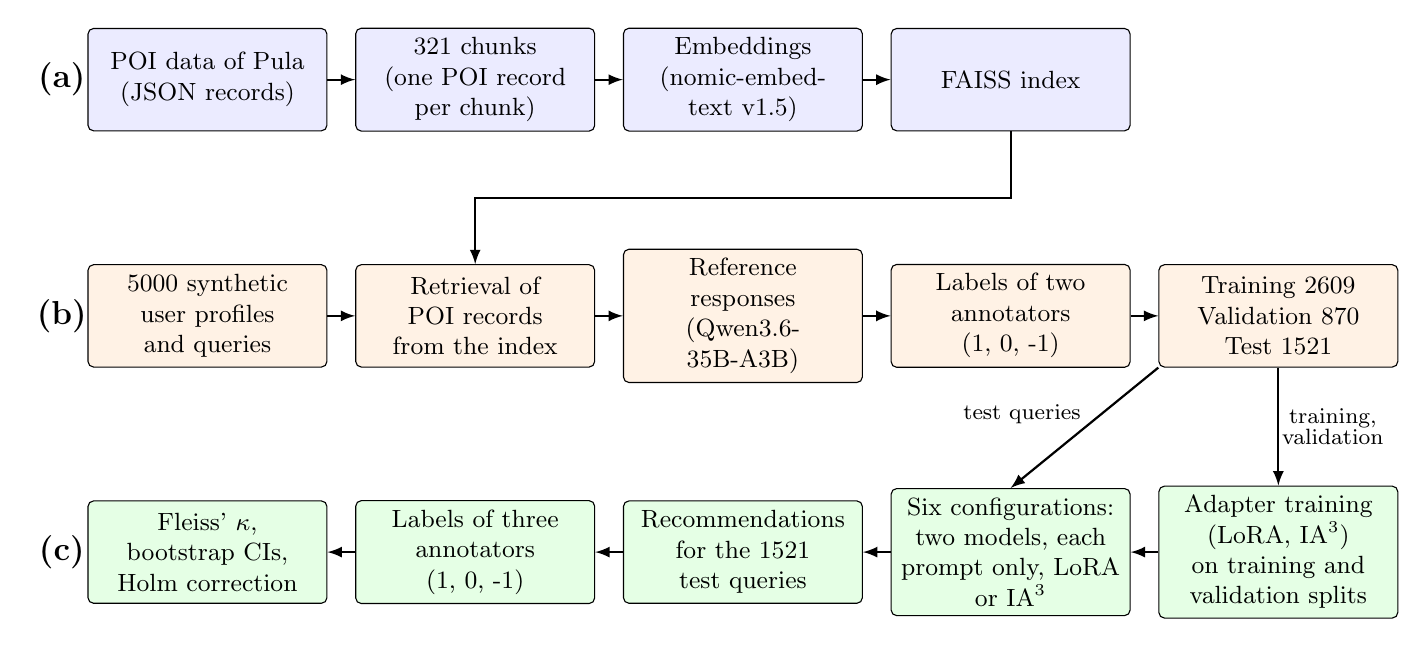
\begin{tikzpicture}[
  font=\small,
  box/.style={draw, rounded corners=2pt, align=center, minimum height=1.3cm, text width=2.8cm, fill=#1},
  box/.default=white,
  arr/.style={->, >=latex, thick},
  lab/.style={font=\large\bfseries},
  note/.style={font=\footnotesize, fill=white, inner sep=1pt, align=center}
]
% Row (a): data preparation
\node[lab] at (-1.85,0) {(a)};
\node[box=blue!8] (poi) at (0,0) {POI data of Pula\\(JSON records)};
\node[box=blue!8] (chunk) at (3.4,0) {321 chunks\\(one POI record\\per chunk)};
\node[box=blue!8] (emb) at (6.8,0) {Embeddings\\(nomic-embed-text v1.5)};
\node[box=blue!8] (idx) at (10.2,0) {FAISS index};
\draw[arr] (poi) -- (chunk); \draw[arr] (chunk) -- (emb); \draw[arr] (emb) -- (idx);
% Row (b): reference responses and splits
\node[lab] at (-1.85,-3) {(b)};
\node[box=orange!10] (prof) at (0,-3) {5000 synthetic\\user profiles\\and queries};
\node[box=orange!10] (ret1) at (3.4,-3) {Retrieval of\\POI records\\from the index};
\node[box=orange!10] (qwen) at (6.8,-3) {Reference responses\\(Qwen3.6-35B-A3B)};
\node[box=orange!10] (ann2) at (10.2,-3) {Labels of two\\annotators\\($1$, $0$, -1)};
\node[box=orange!10] (split) at (13.6,-3) {Training 2609\\Validation 870\\Test 1521};
\draw[arr] (prof) -- (ret1); \draw[arr] (ret1) -- (qwen); \draw[arr] (qwen) -- (ann2); \draw[arr] (ann2) -- (split);
\draw[arr] (idx.south) -- (10.2,-1.5) -- (3.4,-1.5) -- (ret1.north);
% Row (c): adaptation and evaluation
\node[lab] at (-1.85,-6) {(c)};
\node[box=green!10] (train) at (13.6,-6) {Adapter training\\(LoRA, IA$^3$)\\on training and\\validation splits};
\node[box=green!10] (conf) at (10.2,-6) {Six configurations:\\two models, each\\prompt only, LoRA\\or IA$^3$};
\node[box=green!10] (rec) at (6.8,-6) {Recommendations\\for the 1521\\test queries};
\node[box=green!10] (ann3) at (3.4,-6) {Labels of three\\annotators\\($1$, $0$, -1)};
\node[box=green!10] (kap) at (0,-6) {Fleiss' $\kappa$,\\bootstrap CIs,\\Holm correction};
\draw[arr] (split) -- node[note, right] {training,\\[-2pt] validation} (train);
\draw[arr] (split.south west) -- node[note, above left] {test queries} (conf.north);
\draw[arr] (train) -- (conf);
\draw[arr] (conf) -- (rec); \draw[arr] (rec) -- (ann3); \draw[arr] (ann3) -- (kap);
\end{tikzpicture}}
\caption{Pipeline of the study. (\textbf{a}) The POI records of Pula are split into chunks, embedded and stored in a FAISS index. (\textbf{b}) For each of the 5000 synthetic user profiles, POI records are retrieved for the user query, Qwen3.6-35B-A3B generates a reference response, and two annotators label it. The labels define the training, validation and test splits. (\textbf{c}) LoRA and IA$^3$ adapters are trained on the training and validation splits. For the test queries, the six configurations (each foundation model with prompt engineering only, with LoRA and with IA$^3$) generate recommendations, which three annotators label. Their agreement is measured with Fleiss' kappa.\label{fig:pipeline}}
\end{adjustwidth}
\end{figure}

\subsection{Data Collection and Vector Indexing}
A dataset of POIs in the city of Pula, Croatia, was collected by web scraping. The final knowledge base contains 321 POIs of 32 types. Table~\ref{tab:poi} shows the ten most frequent types. The 126 gastronomy POIs (restaurants, cafes, fast food places and pubs) are the largest group. The remaining POIs include accommodation, cultural heritage sites and recreational areas.

\begin{table}[H]
\caption{Number of POIs in the knowledge base by type. The ten most frequent types are listed, and all remaining types are grouped as other.}\label{tab:poi}
\newcolumntype{C}{>{\centering\arraybackslash}X}
\begin{tabularx}{\textwidth}{lCC}
\toprule
Type & POIs & Share of all POIs (\%)\\
\midrule
Restaurant & 74 & 23.1\\
Cafe & 34 & 10.6\\
Artwork & 24 & 7.5\\
Fort & 18 & 5.6\\
Information & 18 & 5.6\\
Park & 16 & 5.0\\
Hotel & 16 & 5.0\\
Fast food & 15 & 4.7\\
Attraction & 14 & 4.4\\
Apartment & 14 & 4.4\\
Other & 78 & 24.3\\
\midrule
Total & 321 & 100.0\\
\bottomrule
\end{tabularx}
\end{table}

The collected data were converted to a common JSON schema. Each POI is represented as a single JSON object containing a categorical type and a nested properties dictionary. Each record contains the following fields:

\begin{itemize}[labelsep=2.5mm,topsep=-3pt]
\item Identification and Contact Fields: The name of the POI for all POIs, and, for gastronomy POIs only, its phone number, opening hours and address (street and house number).
\item Taxonomy Tags: An array of descriptors defining the core attributes of the POI, such as cuisine (e.g., mediterranean), dishes (e.g., pizza), dietary options (e.g., vegetarian) and location (e.g., city\_center). For some POIs, the tags are stored as a single text string instead of an array.
\item Binary and Categorical Constraints: For gastronomy POIs, features such as outdoor\_seating, indoor\_seating, and price (low, medium or high) that describe the practical constraints of the POI.
\item Contextual Narratives: A textual description, a numeric rating and a list of user reviews, which describe the opinions of visitors and the atmosphere of the place.
\end{itemize}\vspace{3pt}

Not every field is available for every POI. Missing values are stored as null. Tags are available for 295 of the 321 POIs, descriptions for 254, ratings for 229 and user reviews for 222. Ratings are between 2.5 and 5.0. A POI has between one and five reviews, most often three. Among the 126 gastronomy POIs, the price is available for 91, the phone number for 108 and the opening hours for 111.

Each JSON object was treated as an independent document chunk, which gives 321 chunks. To enable dense retrieval, embeddings were generated with the nomic-embed-text v1.5 model. The resulting vectors were indexed with Facebook AI Similarity Search (FAISS) for similarity search.

\subsection{Synthetic User Profile Generation and Annotation of Reference Responses}\label{sec:reference}
Evaluating personalized recommendations requires user profiles with varied intents and constraints. We synthetically generated 5000 unique user profiles. Each profile represents a distinct combination of demographic and behavioral traits, mapped to the JSON schema:

\begin{itemize}[labelsep=2.5mm,topsep=-3pt]
\item Demographics: gender, age, and nationality to simulate cultural and generational variance.
\item Behavioral Archetypes: travel\_style (e.g., backpacker, luxury) and persona (e.g., pet\_owner) to establish the user's primary motivation.
\item Explicit Preferences: likes and dislikes structured as arrays of venue tags that describe what the user wants and wants to avoid.
\item Quantitative Constraints: price\_preference and min\_rating that limit which POIs are acceptable.
\item Natural Language Query (input): A conversational prompt synthesized from the profile's constraints (e.g., ``Any nice outdoor spots where I can bring my pet?'').
\end{itemize}\vspace{3pt}

To obtain reference responses for training and evaluation, the Qwen3.6-35B-A3B model generated an initial recommendation response for each of the 5000 queries. Because personalized recommendation is subjective, two annotators checked whether each response met the explicit constraints of the user profile.

The annotators independently marked every response with 1 (agree), 0 (neither) or -1 (disagree). These two annotators were different from the three annotators who rated the outputs of the six configurations on the test split (Section~\ref{sec:eval}). Agreement between the two annotators was low. Of the 5000 responses, 4995 received a valid label from both annotators. On these responses, Cohen's kappa \citep{cohen1960coefficient} was -0.001, which is agreement no better than chance. One annotator marked 96.6\% of the responses with 1 and the other 72.1\%, and the two annotators gave the same label to 70.3\% of the responses. Using only the responses that both annotators marked with 1 for training and validation is therefore a stricter selection than the judgment of either annotator alone. These labels were used to divide the dataset into training, validation and test splits, as described in Section~\ref{sec:dataset}.

\subsection{Dataset Composition and Splits}\label{sec:dataset}
The dataset is synthetic: the 5000 user profiles and their queries were generated and were not collected from real users. The dataset contains 5000 records, one for each synthetic user profile. Each record contains the profile fields (user identifier, name, age, gender, nationality, travel style, persona, likes, dislikes, price preference and minimum rating), the natural language query, the retrieved local information, the initial response generated by Qwen3.6-35B-A3B, and the annotator labels. The retrieved local information is a numbered list of POI records in the JSON format described above, each with its type and its properties. The records were divided into three splits that do not overlap, based on the labels given by the two annotators. Table~\ref{tab:splits} shows the number of queries and the selection rule for each split.

\begin{table}[H]
\caption{Splits of the dataset.}\label{tab:splits}
\newcolumntype{C}{>{\centering\arraybackslash}X}
\begin{tabularx}{\textwidth}{lCCXX}
\toprule
Split & Queries & Share of dataset (\%) & Selection rule & Use\\
\midrule
Training & 2609 & 52.2 & Both annotators marked 1 & Training of the adapters\\
Validation & 870 & 17.4 & Both annotators marked 1 & Validation of the adapters\\
Test & 1521 & 30.4 & At least one of the two annotators did not mark 1 & Evaluation of the six configurations\\
\bottomrule
\end{tabularx}
\end{table}

The 3479 queries that both annotators marked with 1 were divided between training and validation in a ratio of 75:25. The queries were ordered by user identifier: the first 2609 (identifiers 1--3795) formed the training split, and the remaining 870 (identifiers 3797--5000) formed the validation split. Because the identifiers were assigned in the random order in which the profiles were generated, an identifier carries no information about the profile. The shares of personas, travel styles and price preferences differ by at most 2.5 percentage points between the two splits.

The training and validation splits therefore contain only responses that both annotators accepted. The test split contains the remaining queries, whose responses at least one annotator did not accept. All six configurations were evaluated on the test split. The models without adapters did not use the training or validation splits.

\subsection{Retrieval and Context Injection Pipeline}
During inference, a standardized retrieval pipeline is maintained across all evaluated models to isolate the impact of the LLM adaptation strategy. For a given user input, the query is embedded and searched against the FAISS index. The five chunks with the smallest vector distance are retrieved, and these five JSON chunks are injected directly into the LLM prompt.

\subsection{LLM Adaptation Strategies}
The study compares a prompt engineering baseline with two PEFT methods:

\begin{itemize}[labelsep=2.5mm,topsep=-3pt]
\item Prompt Engineering (Baseline): The foundation models receive the same system prompt and user prompt as the configurations with adapters (Section~\ref{sec:inference}), but no adapter is loaded. It uses the five retrieved chunks through in-context learning, without changing the model weights.
\item PEFT: The models are fine-tuned on the training split with two adapter types:
\begin{itemize}[labelsep=2.5mm,topsep=-3pt]
\item LoRA: Freezes the pre-trained model weights and adds trainable low-rank matrices to the layers of the transformer, so that only these matrices are trained.
\item IA$^3$: Scales inner activations with learned vectors and trains far fewer parameters than LoRA.
\end{itemize}\vspace{3pt}
\end{itemize}\vspace{3pt}

\subsection{Adapter Training Configuration}\label{sec:training}
Both adapter types were trained with the same procedure and the same hyperparameters. Each training example was formatted with the chat template of the foundation model and consisted of the system prompt, the user prompt (user profile, user question and retrieved local information) and the target response. The target response was the response generated by Qwen3.6-35B-A3B that both annotators had marked with 1. The 2609 queries of the training split were used to train the adapters, and the 870 queries of the validation split were used to monitor the training. The adapters were trained with the supervised fine-tuning trainer of the Transformer Reinforcement Learning (TRL) library and the PEFT library. Training used two NVIDIA A100 graphics processing units (GPUs). During training, the foundation models were loaded in bfloat16 precision without quantization. Table~\ref{tab:train_shared} lists the settings shared by both adapter types.

\begin{table}[H]
\caption{Training settings shared by the LoRA and IA$^3$ adapters.}\label{tab:train_shared}
\newcolumntype{C}{>{\centering\arraybackslash}X}
\begin{tabularx}{\textwidth}{XC}
\toprule
Setting & Value\\
\midrule
Number of epochs & 3\\
Learning rate & $2 \times 10^{-4}$\\
Learning rate schedule & Linear decay after warmup\\
Warmup ratio & 0.03\\
Optimizer & AdamW\\
Weight decay & 0\\
Gradient clipping (maximum norm) & 1.0\\
Batch size per GPU & 1\\
Gradient accumulation steps & 8\\
Number of GPUs & 2\\
GPU type & NVIDIA A100\\
Effective batch size & 16\\
Maximum sequence length (tokens) & 512\\
Numerical precision & bfloat16\\
Gradient checkpointing & Yes\\
Random seed & 42\\
\bottomrule
\end{tabularx}
\end{table}

The effective batch size was 16 examples, which is a batch size of 1 on each of the two NVIDIA A100 GPUs multiplied by 8 gradient accumulation steps. The validation loss was calculated every 50 steps, and a checkpoint was saved at the same interval. The checkpoint with the lowest validation loss was used as the final adapter. The length of the training examples was measured with the Llama 3 tokenizer, including the chat template. Because the POI records retrieved during training were not stored, the length of the retrieved records was estimated from the records that the same retrieval code returned for the 1521 test queries. On this basis, a training example contained on average about 1790 tokens, and the longest examples about 3400 tokens. Examples longer than the maximum sequence length of 512 tokens were truncated from the end. Even with the five shortest POI records in the knowledge base, 2605 of the 2609 training examples and 864 of the 870 validation examples would be longer than 512 tokens, so at least this many examples were truncated. In almost all examples, the system prompt, the user prompt and the retrieved records alone were longer than 512 tokens, so the reference response was not part of the truncated sequence. The loss was computed over the whole sequence, not only over the response. Table~\ref{tab:train_adapter} lists the settings that are specific to each adapter type.

\begin{table}[H]
\caption{Settings specific to each adapter type.}\label{tab:train_adapter}
\newcolumntype{C}{>{\centering\arraybackslash}X}
\begin{tabularx}{\textwidth}{lXX}
\toprule
Setting & LoRA & IA$^3$\\
\midrule
Rank & 32 & Not applicable\\
Scaling factor (alpha) & 64 & Not applicable\\
Dropout & 0.05 & Not applicable\\
Bias & None & Not applicable\\
Target modules & q\_proj, k\_proj, v\_proj, o\_proj, gate\_proj, up\_proj, down\_proj & k\_proj, v\_proj, down\_proj\\
Feed-forward modules & Not applicable & down\_proj\\
\bottomrule
\end{tabularx}
\end{table}

LoRA was applied to all attention and feed-forward projection layers of the transformer blocks, with trainable matrices of rank 32. IA$^3$ was applied only to the key, value and down projection layers. It trains one scaling vector for each of these layers, which rescales the outputs of the key and value projections and the input of the down projection, so it has far fewer trainable parameters than LoRA. At inference, the trained adapters were applied to foundation models loaded with 4-bit quantization (Section~\ref{sec:inference}).

Table~\ref{tab:train_results} shows the number of trainable parameters, the training time and the final losses for the four adapters. The checkpoint with the lowest validation loss was the last checkpoint for all four adapters.

\begin{table}[H]
\caption{Trainable parameters, training time, final training loss and validation loss of the four adapters. The training time is given in minutes.}\label{tab:train_results}
\newcolumntype{C}{>{\centering\arraybackslash}X}
\begin{tabularx}{\textwidth}{XCCCC}
\toprule
Configuration & Trainable parameters & Training time (min) & Training loss & Validation loss\\
\midrule
Llama 3.1 8B (LoRA) & 83,886,080 & 28.5 & 0.088 & 0.102\\
Llama 3.1 8B (IA$^3$) & 524,288 & 16.2 & 1.385 & 1.421\\
Llama 3.2 3B (LoRA) & 48,627,712 & 24.5 & 0.094 & 0.108\\
Llama 3.2 3B (IA$^3$) & 286,720 & 12.5 & 1.832 & 1.878\\
\bottomrule
\end{tabularx}
\end{table}

Training took between 12.5 and 28.5 minutes. LoRA has about 160 times more trainable parameters than IA$^3$ for Llama 3.1 8B and about 170 times more for Llama 3.2 3B. The loss values of the LoRA adapters (about 0.1) are much lower than those of the IA$^3$ adapters (1.4 and 1.9).

\subsection{Prompt Format and Inference Setup}\label{sec:inference}
All six configurations received the same system prompt and the same user prompt format. The system prompt instructs the model to act as a tourism assistant that recommends personalized activities based on the interests in the user profile, the current question of the user, and the local information retrieved by semantic search. It also instructs the model to respect strong user preferences and to answer with a short and clear activity recommendation, followed by a brief explanation if needed. The user prompt contains the user profile (name, travel style, persona, likes, dislikes, price preference and minimum rating), the user question, and the retrieved local information as a numbered list of POI records. The full system prompt and the template of the user prompt are given in Appendix~\ref{app:prompts}.

At inference, all foundation models were loaded with 4-bit NormalFloat (NF4) quantization and double quantization, while the adapters had been trained on the foundation models loaded in bfloat16 without quantization (Section~\ref{sec:training}). For the configurations with adapters, the trained LoRA or IA$^3$ adapter was loaded on top of the quantized foundation model. The computations were done in bfloat16 for the prompt-only configurations and in float16 for the configurations with adapters. All recommendations were generated with greedy decoding, so the outputs do not depend on a sampling temperature or a random seed. For the prompt-only configurations, the response was limited to 512 new tokens. For the configurations with adapters, no limit on the number of new tokens was set, so generation stopped when the model produced its end-of-sequence token or reached its context length.

\subsection{Evaluation Protocol and Inter-Rater Agreement}\label{sec:eval}
Six configurations were evaluated: Llama 3.1 8B and Llama 3.2 3B, each under prompt engineering, LoRA and IA$^3$. Each configuration is named after the foundation model, followed by the adaptation strategy in parentheses: Llama 3.1 8B (prompt only), Llama 3.1 8B (LoRA) and Llama 3.1 8B (IA$^3$), and the same for Llama 3.2 3B. Each configuration generated recommendations for the same set of 1521 test queries. The same three annotators rated all recommendations. They were volunteer students of the Faculty of Informatics, Juraj Dobrila University of Pula, who know the city and have basic knowledge of computer science. They were not told which model or adaptation method produced each recommendation. The annotators were asked to judge whether each recommendation suited the user profile. For example, a user who dislikes meat and asks for a restaurant has to be recommended a place that serves meals without meat, and a user who likes a family environment has to be recommended places that are suitable for families. For every recommendation, the three annotators independently assigned one of three labels: 1 (the annotator agrees with the recommendation), -1 (the annotator disagrees) or 0 (neither). Since no objective ground truth exists for subjective recommendation quality, the evaluation relies on the consistency of these independent judgments, quantified with Fleiss' kappa \citep{fleiss1971measuring}.

Let $N$ be the number of evaluated recommendations, $n=3$ the number of annotators, $k=3$ the number of categories, and $n_{ij}$ the number of annotators who assigned recommendation $i$ to category $j$. The observed agreement for a single recommendation and its mean are

\begin{equation}
P_i = \frac{1}{n(n-1)}\left(\sum_{j=1}^{k} n_{ij}^{2} - n\right), \qquad \bar{P} = \frac{1}{N}\sum_{i=1}^{N} P_i .
\end{equation}

The expected chance agreement is computed from the overall proportion $p_j$ of ratings in each category, and Fleiss' kappa follows as

\begin{equation}
p_j = \frac{1}{Nn}\sum_{i=1}^{N} n_{ij}, \qquad \bar{P}_e = \sum_{j=1}^{k} p_j^{2}, \qquad \kappa = \frac{\bar{P} - \bar{P}_e}{1 - \bar{P}_e}.
\end{equation}

A value of $\kappa = 1$ indicates perfect agreement, while $\kappa = 0$ indicates agreement no better than chance. Values are interpreted using the scale of Landis and Koch \citep{landis1977measurement}: slight (0.01--0.20), fair (0.21--0.40), moderate (0.41--0.60), substantial (0.61--0.80) and almost perfect (0.81--1.00) agreement. Fleiss' kappa expresses how consistently annotators judge the recommendations, not whether the judgments are correct. Uncertainty was estimated by nonparametric bootstrap, resampling queries with replacement (20,000 replicates) and reporting 95\% percentile intervals. Nine comparisons were planned: each adapter configuration against the same model without an adapter (four comparisons), LoRA against IA$^3$ for each model (two comparisons), and the same configuration (without adapter, with LoRA and with IA$^3$) on the two foundation models (three comparisons). The differences in kappa were estimated with a paired bootstrap on the same resampled queries. Because nine comparisons were made, the two-sided p-values were adjusted with the Holm method, which reduces the chance of false positive findings when several comparisons are tested together.

\subsection{Analysis of the Generated Responses}\label{sec:output_method}
After the annotation, the generated responses were checked automatically for two problems that the agreement measure does not capture. A response was counted as containing copied POI records if it contained one of the strings \texttt{"reviews"}, \texttt{"properties"}, \texttt{\{"type"} or \texttt{]\}}. These strings occur in the JSON records of the knowledge base but not in normal text. A response was counted as unfinished if its last character was not a period, a question mark, an exclamation mark, a closing bracket, an asterisk or a quotation mark. Both checks are simple text rules. They can miss some cases, and the second rule can count a response that ends with a list item as unfinished. For the configurations with copied records, the share of label 1 was compared between the responses with and without copied records. These comparisons are descriptive and were not tested statistically.

%%%%%%%%%%%%%%%%%%%%%%%%%%%%%%%%%%%%%%%%%%
\section{Results and Discussion}\label{sec:results}

This section reports the inter-rater agreement for the six configurations on the test set of 1521 queries. Three annotators rated each recommendation, which gives 4563 ratings for each configuration. The results are presented in five parts: the agreement for each configuration, the distribution of the labels, the comparison of the adaptation strategies, the analysis of the generated responses, and a discussion of the findings.

\subsection{Agreement for Each Configuration}
Table~\ref{tab:kappa} shows Fleiss' kappa, its 95\% confidence interval, the observed agreement $\bar{P}$ and the chance agreement $\bar{P}_e$ for each configuration. Figure~\ref{fig:kappa} shows the kappa values.

\begin{table}[H]
\caption{Fleiss' kappa ($\kappa$), 95\% bootstrap confidence interval (CI), observed agreement ($\bar{P}$) and chance agreement ($\bar{P}_e$) for the six configurations on the 1521 test queries.}\label{tab:kappa}
\newcolumntype{C}{>{\centering\arraybackslash}X}
\begin{tabularx}{\textwidth}{lCCCC}
\toprule
Configuration & $\kappa$ & 95\% CI & $\bar{P}$ & $\bar{P}_e$\\
\midrule
Llama 3.1 8B (prompt only) & 0.863 & 0.840 to 0.884 & 0.926 & 0.464\\
Llama 3.1 8B (LoRA) & 0.902 & 0.882 to 0.920 & 0.950 & 0.487\\
Llama 3.1 8B (IA$^3$) & 0.877 & 0.851 to 0.901 & 0.954 & 0.630\\
Llama 3.2 3B (prompt only) & 0.875 & 0.854 to 0.895 & 0.930 & 0.439\\
Llama 3.2 3B (LoRA) & 0.888 & 0.869 to 0.906 & 0.937 & 0.435\\
Llama 3.2 3B (IA$^3$) & 0.904 & 0.882 to 0.924 & 0.961 & 0.597\\
\bottomrule
\end{tabularx}
\end{table}

Fleiss' kappa was between 0.863 and 0.904 for all six configurations. All values are in the almost perfect range (0.81 to 1.00) of the scale used in this study. The lower end of the 95\% confidence interval was at least 0.84 for every configuration. Hypothesis H1 is therefore supported: the annotators reached at least substantial agreement under every adaptation strategy.

The observed agreement $\bar{P}$ was between 0.926 and 0.961. The chance agreement $\bar{P}_e$ was between 0.435 and 0.630. Chance agreement is the agreement that would be expected if the annotators gave their labels independently, with the label frequencies of the configuration. Kappa measures how much of the agreement above this level was reached. $\bar{P}_e$ was higher for the two IA$^3$ configurations (0.630 and 0.597) than for the other four configurations (0.435 to 0.487), because label 1 was more frequent for the IA$^3$ configurations (Section~\ref{sec:labels}). For this reason, Llama 3.1 8B (IA$^3$) has the highest observed agreement of the three Llama 3.1 8B configurations (0.954), but a lower kappa (0.877) than Llama 3.1 8B (LoRA) (0.902), which has an observed agreement of 0.950.

\begin{figure}[H]
\centering
\includegraphics[width=12 cm]{figures/fig_kappa.png}
\caption{Fleiss' kappa for the six configurations on the 1521 test queries, grouped by foundation model. The prompt engineering baseline (prompt only) uses the foundation model without an adapter. The error bars show the 95\% bootstrap confidence intervals from Table~\ref{tab:kappa} (20,000 replicates, resampling queries). The value of kappa is printed inside each bar. The vertical axis starts at 0.80.}\label{fig:kappa}
\end{figure}

Figure~\ref{fig:kappa} shows the same kappa values grouped by foundation model. The highest kappa was reached by Llama 3.2 3B (IA$^3$) (0.904), followed closely by Llama 3.1 8B (LoRA) (0.902), and the lowest by Llama 3.1 8B without an adapter (0.863). The differences between the configurations are small. The confidence intervals overlap for all configurations of the same foundation model. Overlapping intervals do not show that two configurations are equal, and the paired comparisons in Section~\ref{sec:comparison} are used to test the differences between configurations, because they take into account that every configuration was rated on the same queries.

\subsection{Distribution of the Labels}\label{sec:labels}
Table~\ref{tab:labels} shows how often each label was used. These counts are descriptive. They are reported to show what the annotators decided and to explain the chance agreement in Table~\ref{tab:kappa}.

\begin{table}[H]
\caption{Number of ratings for each label and, in brackets, their share of the 4563 ratings given to each configuration (three annotators, 1521 queries), in percent.}\label{tab:labels}
\newcolumntype{C}{>{\centering\arraybackslash}X}
\begin{tabularx}{\textwidth}{lCCC}
\toprule
Configuration & Label 1 (agree) & Label 0 (neither) & Label -1 (disagree)\\
\midrule
Llama 3.1 8B (prompt only) & 2720 (59.6) & 389 (8.5) & 1454 (31.9)\\
Llama 3.1 8B (LoRA) & 2862 (62.7) & 346 (7.6) & 1355 (29.7)\\
Llama 3.1 8B (IA$^3$) & 3544 (77.7) & 389 (8.5) & 630 (13.8)\\
Llama 3.2 3B (prompt only) & 2534 (55.5) & 441 (9.7) & 1588 (34.8)\\
Llama 3.2 3B (LoRA) & 2449 (53.7) & 417 (9.1) & 1697 (37.2)\\
Llama 3.2 3B (IA$^3$) & 3414 (74.8) & 337 (7.4) & 812 (17.8)\\
\bottomrule
\end{tabularx}
\end{table}

Label 1 was given to 77.7\% of the ratings for Llama 3.1 8B (IA$^3$) and to 74.8\% for Llama 3.2 3B (IA$^3$). For the other four configurations, the share of label 1 was between 53.7\% and 62.7\%. Label -1 showed the opposite pattern: 13.8\% and 17.8\% for the two IA$^3$ configurations, and between 29.7\% and 37.2\% for the other four. Label 0 was used for between 7.4\% and 9.7\% of the ratings in every configuration. LoRA increased the share of label 1 for Llama 3.1 8B (62.7\% compared with 59.6\%) but not for Llama 3.2 3B (53.7\% compared with 55.5\%).

These shares were not tested statistically, and Fleiss' kappa does not measure them. They show that the annotators agreed with the recommendations of the IA$^3$ configurations more often than with those of the other configurations. This may mean that the IA$^3$ recommendations matched the user profiles better, but this study did not test it.

\subsection{Comparison of the Adaptation Strategies}\label{sec:comparison}
Table~\ref{tab:comparisons} shows the nine planned comparisons. Each difference is the kappa of the configuration in the first column minus the kappa of the configuration in the second column, so a positive value means that the configuration in the first column has the higher kappa.

\begin{table}[H]
\begin{adjustwidth}{-\extralength}{0cm}
\caption{Planned comparisons. Difference in Fleiss' kappa between the configuration in the first column and the configuration in the second column, its 95\% bootstrap confidence interval (CI) and the p-value adjusted with the Holm method for nine comparisons. The confidence intervals are not adjusted for multiple comparisons.}\label{tab:comparisons}
\newcolumntype{C}{>{\centering\arraybackslash}X}
\begin{tabularx}{\fulllength}{llCCC}
\toprule
Configuration & Compared with & Difference in $\kappa$ & 95\% CI & Adjusted p\\
\midrule
Llama 3.1 8B (LoRA) & Llama 3.1 8B (prompt only) & 0.039 & 0.014 to 0.064 & 0.015\\
Llama 3.1 8B (IA$^3$) & Llama 3.1 8B (prompt only) & 0.014 & -0.016 to 0.044 & 0.878\\
Llama 3.2 3B (LoRA) & Llama 3.2 3B (prompt only) & 0.013 & -0.011 to 0.037 & 0.878\\
Llama 3.2 3B (IA$^3$) & Llama 3.2 3B (prompt only) & 0.029 & 0.002 to 0.055 & 0.262\\
Llama 3.1 8B (LoRA) & Llama 3.1 8B (IA$^3$) & 0.025 & -0.003 to 0.053 & 0.458\\
Llama 3.2 3B (LoRA) & Llama 3.2 3B (IA$^3$) & -0.016 & -0.034 to 0.003 & 0.458\\
Llama 3.1 8B (prompt only) & Llama 3.2 3B (prompt only) & -0.012 & -0.037 to 0.012 & 0.878\\
Llama 3.1 8B (LoRA) & Llama 3.2 3B (LoRA) & 0.014 & -0.006 to 0.033 & 0.717\\
Llama 3.1 8B (IA$^3$) & Llama 3.2 3B (IA$^3$) & -0.027 & -0.056 to 0.001 & 0.411\\
\bottomrule
\end{tabularx}
\end{adjustwidth}
\end{table}

Hypothesis H2 expected that the models with adapters would be judged more consistently than the same models without adapters. All four adapter configurations had a higher kappa than the model without an adapter, with differences between 0.013 and 0.039. After the Holm correction, only the difference for LoRA on Llama 3.1 8B was statistically significant (0.039, 95\% CI 0.014 to 0.064, adjusted p = 0.015). The difference for IA$^3$ on Llama 3.2 3B (0.029) had an unadjusted p-value of 0.033 and an adjusted p-value of 0.262. H2 is therefore only partially supported: all four differences have the expected direction, but only one of them is statistically significant after the Holm correction.

Hypothesis H3 expected that LoRA would reach a higher agreement than IA$^3$. LoRA had a higher kappa on Llama 3.1 8B (0.025) and a lower kappa on Llama 3.2 3B (-0.016). Neither difference was statistically significant (adjusted p = 0.458 for both). H3 is not supported.

Hypothesis H4 expected the same order of the strategies for both foundation models. The model without an adapter had the lowest kappa of its three configurations for both Llama 3.1 8B and Llama 3.2 3B. The order of LoRA and IA$^3$ was different for the two models. The same configuration did not differ significantly between the two foundation models: the differences (Llama 3.1 8B minus Llama 3.2 3B) were -0.012 without an adapter, 0.014 with LoRA and -0.027 with IA$^3$, with adjusted p-values between 0.411 and 0.878. The difference between the LoRA and IA$^3$ results was 0.041 larger for Llama 3.1 8B than for Llama 3.2 3B (95\% CI 0.008 to 0.074). This comparison was not one of the nine planned comparisons and was not adjusted. H4 is therefore supported for the position of the model without an adapter, but not for the order of the two adapters.

\subsection{Analysis of the Generated Responses}\label{sec:outputs}
Table~\ref{tab:outputs} shows how many responses of each configuration contained copied POI records and how many were unfinished, according to the checks described in Section~\ref{sec:output_method}.

\begin{table}[H]
\caption{Responses with copied POI records and unfinished responses for each configuration, out of 1521 responses per configuration, with the share in percent in brackets. A response can have both problems, so the last column counts the responses with at least one of them.\label{tab:outputs}}
\newcolumntype{C}{>{\centering\arraybackslash}X}
\begin{tabularx}{\textwidth}{lCCC}
\toprule
Configuration & Copied POI records & Unfinished & At least one\\
\midrule
Llama 3.1 8B (prompt only) & 0 (0.0) & 81 (5.3) & 81 (5.3)\\
Llama 3.1 8B (LoRA) & 300 (19.7) & 382 (25.1) & 410 (27.0)\\
Llama 3.1 8B (IA$^3$) & 0 (0.0) & 258 (17.0) & 258 (17.0)\\
Llama 3.2 3B (prompt only) & 0 (0.0) & 119 (7.8) & 119 (7.8)\\
Llama 3.2 3B (LoRA) & 1116 (73.4) & 880 (57.9) & 1148 (75.5)\\
Llama 3.2 3B (IA$^3$) & 4 (0.3) & 157 (10.3) & 157 (10.3)\\
\bottomrule
\end{tabularx}
\end{table}

No response of the two prompt-only configurations contained copied POI records. Copied records appeared in 19.7\% of the responses of Llama 3.1 8B (LoRA) and in 73.4\% of the responses of Llama 3.2 3B (LoRA), but in none of the responses of Llama 3.1 8B (IA$^3$) and in only 4 responses of Llama 3.2 3B (IA$^3$). Unfinished responses were least frequent for the prompt-only configurations (5.3\% and 7.8\%), more frequent for the IA$^3$ configurations (17.0\% and 10.3\%), and most frequent for the LoRA configurations (25.1\% and 57.9\%). For Llama 3.2 3B (LoRA), 848 of the 1116 responses with copied records were also unfinished.

The annotators often agreed with responses that contained copied records. For Llama 3.1 8B (LoRA), label 1 was given to 56.8\% of the ratings of responses with copied records and to 64.2\% of the ratings of responses without them. For Llama 3.2 3B (LoRA), the shares were 51.1\% and 60.7\%. The unfinished responses of the IA$^3$ configurations received label 1 in 76.6\% (Llama 3.1 8B) and 70.3\% (Llama 3.2 3B) of the ratings.

\subsection{Discussion}\label{sec:discussion}
The annotators reached almost perfect agreement for all six configurations. The test set contained only queries for which the annotators had not all marked the initial response with 1 during the annotation of the reference responses. Even so, the observed agreement for the recommendations of the six configurations was between 0.926 and 0.961. The annotators did not know which configuration produced each recommendation, so the agreement does not depend on knowledge of the model.

The differences in kappa between configurations were small, at most 0.041. No adapter configuration had a lower kappa than the same model without an adapter. Using LoRA or IA$^3$ therefore did not make the recommendations harder to judge consistently. The only difference that remained statistically significant after correction was LoRA on Llama 3.1 8B. There was no consistent difference between LoRA and IA$^3$, because the better adapter was not the same for the two foundation models. The same configuration also did not differ significantly between Llama 3.1 8B and Llama 3.2 3B.

The results for the IA$^3$ configurations show that kappa should be read together with the label distribution. These configurations received label 1 more often, which raised the chance agreement and lowered kappa relative to the observed agreement. Kappa measures how consistently the annotators judged the recommendations. It does not measure how accurate the recommendations are, so a higher kappa for one configuration does not show that its recommendations are better. The label shares in Table~\ref{tab:labels} point towards the IA$^3$ configurations as the ones whose recommendations the annotators accepted most often. A statistical test of the label shares is needed to confirm this.

The label shares also show a result that needs an explanation. The LoRA configurations received label 1 less often than the IA$^3$ configurations, although LoRA trains about 160 to 170 times more parameters, and Llama 3.2 3B (LoRA) received label 1 less often (53.7\%) than the same model without an adapter (55.5\%).

The most likely explanation is the truncation of the training examples (Section~\ref{sec:training}). The examples averaged about 1790 tokens, but only the first 512 tokens were used, and in almost all examples these tokens contained only the system prompt, the user prompt and part of the retrieved POI records. The reference response was therefore almost never part of the training text. Because the loss was computed over the whole sequence, the adapters were trained to continue the prompt and the POI records rather than to write a recommendation. The responses show the result of this training (Table~\ref{tab:outputs}). LoRA, which changes the weights of all seven projection layers, learned to reproduce the JSON records: 73.4\% of the responses of Llama 3.2 3B (LoRA) and 19.7\% of those of Llama 3.1 8B (LoRA) contained copied records. IA$^3$, which only rescales the activations of three layer types, almost never did. The training losses agree with this explanation. The LoRA adapters reached a loss of about 0.1 on the truncated sequences, which consist mostly of the same system prompt and of records of the same 321 POIs, while the IA$^3$ adapters stayed at 1.4 and 1.9 (Table~\ref{tab:train_results}). The validation examples were truncated in the same way, so the validation loss could not show that the adapters did not learn to write responses.

Under these training conditions, IA$^3$ appears to have kept the ability of the foundation models to write a recommendation, and its configurations received label 1 most often. LoRA changed the behavior of the foundation models more strongly, and for the smaller model this change came with a lower share of label 1 than without an adapter. These results describe adapters trained on truncated sequences. They do not show how LoRA and IA$^3$ compare when the full reference responses are part of the training text, and the study cannot separate the effect of the adapter type from the effect of the truncation.

Two other factors may have contributed. First, the adapters were trained on the foundation models in bfloat16 precision and applied to the same models with 4-bit quantization (Section~\ref{sec:inference}). LoRA adds a learned update to the weights, which may be affected more by this difference than the scaling vectors of IA$^3$. Second, the training and validation splits contain only queries whose reference responses both annotators accepted, while the test split contains the remaining queries, so the adapters were tested on a different kind of query than they were trained on. Neither factor explains the copied POI records, which appear only in the adapter configurations.

The analysis of the responses also shows a limit of the evaluation by agreement. The annotators gave label 1 to 56.8\% and 51.1\% of the ratings of LoRA responses that contained copied POI records. The annotators were asked to judge whether a recommendation suited the user profile, and a response that names a suitable place and then continues with copied records can meet this condition. High agreement and a high share of label 1 therefore do not show that a response is usable in an application. An automatic check of the output, such as the checks in Section~\ref{sec:output_method}, adds information that the human labels did not capture.

Three practical lessons follow. First, the length of the training examples should be measured with the tokenizer of the model before training, and the maximum sequence length should cover the full example, including the response. Prompts that contain retrieved JSON records are long, and in this study the prompt alone was longer than 512 tokens in almost all examples. Second, the loss should be computed only on the tokens of the response, so that a truncated example does not train the adapter on the prompt. Third, the generated responses should be checked for format problems in addition to the human evaluation.

Some limits apply to these results. The recommendations are for one city, Pula, and were rated by three annotators. The test set contains only the queries that were difficult during annotation, and the label shares were not tested statistically. These and other limits are discussed in Section~\ref{sec:limitations}.

%%%%%%%%%%%%%%%%%%%%%%%%%%%%%%%%%%%%%%%%%%
\section{Limitations and Future Work}\label{sec:limitations}

This section describes the limitations of the study and proposes directions for future work. The limitations concern the evaluation measure, the data, the models and training, and the settings used for inference. The future work follows from these limitations.

\subsection{Limitations}
The most important limitation is the truncation of the training examples. The maximum sequence length of 512 tokens was much shorter than the training examples, which averaged about 1790 tokens, so the reference response was cut off in almost all of them (Section~\ref{sec:training}). The adapters were therefore trained mostly on the prompt and the retrieved records, not on the reference responses. With a maximum sequence length that covers the full examples and a loss computed only on the response, the adapters may behave differently, and the differences between LoRA, IA$^3$ and prompt engineering may change in size or direction. The adapters were not retrained to test this. The checks for copied records and unfinished responses are simple text rules and may miss some cases.

The evaluation in this study is based on Fleiss' kappa, which measures how consistently the three annotators judged the recommendations. A high kappa shows that the annotators agreed with each other. It does not show that a recommendation is correct or that its quality is high. Personalized recommendation is subjective, and no objective ground truth exists. The shares of the labels in Table~\ref{tab:labels} were reported only as descriptive counts and were not tested statistically. For this reason, the study cannot state which configuration gives better recommendations.

Only responses that both annotators marked with 1 were used for training and validation. The agreement between these two annotators was no better than chance (Cohen's $\kappa =$ -0.001, Section~\ref{sec:reference}), so the selection mainly reflects the judgment of the stricter annotator, and the accepted responses represent the views of two individuals. All training responses were also generated by one model, Qwen3.6-35B-A3B, so the adapters learned from the content and style of a single model. The test set of 1521 queries was used to test the configurations after training. It contains the queries for which the annotators did not all mark the initial response with 1, so these queries may be more difficult and more subjective than the rest of the dataset. The validation split was selected with the same rule as the training split, so the validation loss used to select the checkpoints shows how well an adapter reproduces accepted responses, but not how well it handles difficult queries. The results therefore show how the configurations behave on difficult cases, and they may be different for a random sample of queries.

The user profiles and queries are synthetic. Real users may write their requests in a different way, with different wording, length and level of detail, so the results may not transfer directly to real requests. The knowledge base covers one small city, Pula, with 321 POIs, and the system was not tested on a large city with many more POIs. Each POI is stored as one JSON object that contains all of its fields, and this design may not work as well for a much larger number of POIs. The results could be different for larger cities for this reason.

Only two foundation models were used, Llama 3.1 8B and Llama 3.2 3B, and both belong to the same model family. Each adapter was trained once, with one random seed and one set of hyperparameters, which was the same for LoRA and IA$^3$. The settings were not tuned separately for each adapter type, so a different setting could favor one adapter type. The bootstrap confidence intervals describe the variation between test queries. They do not describe the variation between training runs, which can only be measured by training the same adapter several times.

All six configurations were evaluated with 4-bit quantization, while the adapters were trained on models loaded without quantization. Quantization changes the model weights slightly, so an adapter may behave differently on a quantized model than on the model it was trained on. An evaluation without quantization was not done, and the results may be different at full precision. Finally, the study did not measure inference latency or cost. The training time and the number of trainable parameters were reported, but the time and cost needed to generate recommendations were not compared between the configurations.

\subsection{Future Work}
Several directions follow from these limitations. The first and most direct is to retrain both adapter types with a maximum sequence length that covers the full training examples (up to about 3400 tokens in this dataset) and with the loss computed only on the response, and to repeat the evaluation with the same annotators. This would show how LoRA and IA$^3$ compare when they learn from the reference responses. The second is to test more foundation models, including models from other families and of different sizes, to check whether the results are specific to the two Llama models. The third is to build knowledge bases for other cities, including large cities with many more POIs, and to include more POI types. This would show whether storing each POI as one JSON object and retrieving five chunks still works at a larger scale.

The fourth direction is to train each adapter several times with different random seeds, so that the variation between training runs can be measured and reported together with the variation between test queries. The fifth is to evaluate the configurations with real user profiles and real questions written by people, instead of synthetic data. The sixth is to tune the hyperparameters, such as the rank, the learning rate and the number of epochs, separately for each adapter type, and to evaluate the adapters without quantization. Finally, the human evaluation can be combined with automatic checks of the output format and with a statistical test of how often the annotators accept the recommendations of each configuration, which would add a measure of recommendation quality to the measure of agreement used here.

%%%%%%%%%%%%%%%%%%%%%%%%%%%%%%%%%%%%%%%%%%
\section{Conclusions}\label{sec:conclusions}

This study compared two parameter-efficient fine-tuning methods, LoRA and IA$^3$, with prompt engineering for personalized point-of-interest recommendation in the city of Pula. Llama 3.1 8B and Llama 3.2 3B were used, which gave six configurations. Three annotators rated the recommendations of each configuration for 1521 test queries, without knowing which configuration produced them. Their agreement, measured with Fleiss' kappa, was between 0.863 and 0.904 for all six configurations, which is almost perfect agreement. All four adapter configurations had a higher kappa than the same model without an adapter, but the differences were small, and only Llama 3.1 8B (LoRA) remained statistically significant after correction for multiple comparisons.

The training examples were much longer than the maximum sequence length of 512 tokens, so the reference responses were cut off in almost all of them, and the adapters were trained mostly on the prompt and the retrieved POI records. The two adapter types reacted differently to this. LoRA learned to reproduce the records: 19.7\% and 73.4\% of its responses contained copied JSON records. IA$^3$ almost never did, and its configurations received label 1 most often (77.7\% and 74.8\% of the ratings). The annotators still gave label 1 to more than half of the ratings of LoRA responses with copied records, so agreement and acceptance alone did not reveal this problem.

For fine-tuning on prompts with retrieved records, the length of the training examples should be checked against the maximum sequence length, the loss should be computed only on the response, and the human evaluation should be combined with automatic checks of the output. The study used synthetic profiles and queries, one small city, two Llama models and one training run for each adapter. These limitations and the planned future work are described in Section~\ref{sec:limitations}.

%%%%%%%%%%%%%%%%%%%%%%%%%%%%%%%%%%%%%%%%%%
\vspace{6pt} 

%%%%%%%%%%%%%%%%%%%%%%%%%%%%%%%%%%%%%%%%%%
%% optional
%\supplementary{The following supporting information can be downloaded at:  \linksupplementary{s1}, Figure S1: title; Table S1: title; Video S1: title.}

% Only for journal Methods and Protocols:
% If you wish to submit a video article, please do so with any other supplementary material.
% \supplementary{The following supporting information can be downloaded at: \linksupplementary{s1}, Figure S1: title; Table S1: title; Video S1: title. A supporting video article is available at doi: link.}

% Only used for preprtints:
% \supplementary{The following supporting information can be downloaded at the website of this paper posted on \href{https://www.preprints.org/}{Preprints.org}.}

% Only for journal Hardware:
% If you wish to submit a video article, please do so with any other supplementary material.
% \supplementary{The following supporting information can be downloaded at: \linksupplementary{s1}, Figure S1: title; Table S1: title; Video S1: title.\vspace{6pt}\\
%\begin{tabularx}{\textwidth}{lll}
%\toprule
%\textbf{Name} & \textbf{Type} & \textbf{Description} \\
%\midrule
%S1 & Python script (.py) & Script of python source code used in XX \\
%S2 & Text (.txt) & Script of modelling code used to make Figure X \\
%S3 & Text (.txt) & Raw data from experiment X \\
%S4 & Video (.mp4) & Video demonstrating the hardware in use \\
%... & ... & ... \\
%\bottomrule
%\end{tabularx}
%}

%%%%%%%%%%%%%%%%%%%%%%%%%%%%%%%%%%%%%%%%%%
\authorcontributions{Conceptualization, R.K., L.S. and S.B.Š.; methodology, L.S.; software, L.S.; validation, I.L. and S.B.Š.; formal analysis, R.K.; investigation, R.K. and L.S.; resources, R.K. and V.M.; data curation, R.K. and L.S.; writing—original draft preparation, R.K. and L.S.; writing—review and editing, S.B.Š., I.L., and V.M.; visualization, R.K.; supervision, S.B.Š. and I.L.; project administration, S.B.Š. and I.L.; funding acquisition, V.M. and I.L. All authors have read and agreed to the published version of the manuscript.}

\funding{This work was (partially) supported by the EC Digital Europe Programme EDIH Adria 2.0 (101256325); SPIN projects IP.1.1.03.0120, IP.1.1.03.0158 and IP.1.1.03.0039; and NextGenerationEU University grants: uniri-iz-25-6, uniri-iz-25-220, IIP\_010144, IIP\_010136.}

\institutionalreview{The annotators were volunteer students of the Faculty of Informatics, Juraj Dobrila University of Pula, who participated as annotators of model outputs rather than as research participants. No personal or sensitive data about the annotators were collected, and the user profiles in the dataset are synthetic. No institutional review board approval was required for this study under the applicable national regulations.}

\informedconsent{Informed consent was obtained from all annotators involved in the study. The annotators participated voluntarily and were not compensated.}

% Written informed consent for publication must be obtained from participating patients who can be identified (including by the patients themselves). Please state ``Written informed consent has been obtained from the patient(s) to publish this paper'' if applicable.}

\dataavailability{The original data presented in this study are openly available in a public repository at \url{https://github.com/FIPU-SPIN/lora-tourism-recommender}}

%\durcstatement{Current research is limited to the [please insert a specific academic field, e.g., XXX], which is beneficial [share benefits and/or primary use] and does not pose a threat to public health or national security. Authors acknowledge the dual-use potential of the research involving xxx and confirm that all necessary precautions have been taken to prevent potential misuse. As an ethical responsibility, authors strictly adhere to relevant national and international laws about DURC. Authors advocate for responsible deployment, ethical considerations, regulatory compliance, and transparent reporting to mitigate misuse risks and foster beneficial outcomes.}

% Only for journal Nursing Reports
%\publicinvolvement{Please describe how the public (patients, consumers, carers) were involved in the research. Consider reporting against the GRIPP2 (Guidance for Reporting Involvement of Patients and the Public) checklist. If the public were not involved in any aspect of the research add: ``No public involvement in any aspect of this research''.}
%
%% Only for journal Nursing Reports
%\guidelinesstandards{Please add a statement indicating which reporting guideline was used when drafting the report. For example, ``This manuscript was drafted against the XXX (the full name of reporting guidelines and citation) for XXX (type of research) research''. A complete list of reporting guidelines can be accessed via the equator network: \url{https://www.equator-network.org/}.}
%
%% Only for journal Nursing Reports
%\useofartificialintelligence{Please describe in detail any and all uses of artificial intelligence (AI) or AI-assisted tools used in the preparation of the manuscript. This may include, but is not limited to, language translation, language editing and grammar, or generating text. Alternatively, please state that “AI or AI-assisted tools were not used in drafting any aspect of this manuscript”.}

\acknowledgments{This research was performed using the Advanced computing service provided by the University of Zagreb University Computing Centre (SRCE).}

\conflictsofinterest{The authors declare no conflicts of interest.} 

%%%%%%%%%%%%%%%%%%%%%%%%%%%%%%%%%%%%%%%%%%
%% Optional

%% Only for journal Encyclopedia
%\entrylink{The Link to this entry published on the encyclopedia platform.}

\abbreviations{Abbreviations}{
The following abbreviations are used in this manuscript:
\\

\noindent 
\begin{tabular}{@{}ll}
AdamW & Adaptive Moment Estimation with Decoupled Weight Decay\\
API & Application Programming Interface\\
BERT & Bidirectional Encoder Representations from Transformers\\
bfloat16 & Brain Floating Point 16-bit Format\\
CI & Confidence Interval\\
EC & European Commission\\
EDIH & European Digital Innovation Hub\\
FAISS & Facebook AI Similarity Search\\
GPT & Generative Pre-trained Transformer\\
GPU & Graphics Processing Unit\\
IA$^3$ & Infused Adapter by Inhibiting and Amplifying Inner Activations\\
JSON & JavaScript Object Notation\\
LLM & Large Language Model\\
LoRA & Low-Rank Adaptation\\
NF4 & 4-bit NormalFloat\\
PEFT & Parameter-Efficient Fine-Tuning\\
POI & Point of Interest\\
QLoRA & Quantized Low-Rank Adaptation\\
RAG & Retrieval-Augmented Generation\\
SRCE & University Computing Centre (Croatian: Sveu\v{c}ili\v{s}ni ra\v{c}unski centar)\\
T5 & Text-to-Text Transfer Transformer\\
TRL & Transformer Reinforcement Learning\\
$\kappa$ & Kappa coefficient of agreement (Fleiss' kappa, unless Cohen's kappa is stated)\\
\end{tabular}
}

%%%%%%%%%%%%%%%%%%%%%%%%%%%%%%%%%%%%%%%%%%
\appendixtitles{yes}
\appendixstart
\appendix
\section[\appendixname~\thesection]{Prompts}\label{app:prompts}

This appendix gives the system prompt and the template of the user prompt that were used for training the adapters and for generating the recommendations of all six configurations. In the user prompt, the text in angle brackets is replaced by the values from the user profile, the user question and the retrieved POI records.

\vspace{6pt}
\noindent\textbf{System prompt}

\vspace{3pt}
\noindent\fbox{\parbox{\dimexpr\linewidth-2\fboxsep-2\fboxrule\relax}{\small\ttfamily\raggedright
You are an intelligent tourism assistant. You recommend personalized activities to tourists based on:\\
1. The user's interests and preferences (as defined in their profile).\\
2. Their current intent or question (described in the user input).\\
3. Relevant local information retrieved via semantic search (provided as bullet points).\\
Your response should be personalized, context-aware, and practical.\\
If there are strong user preferences, make sure to respect them.\\
Respond in a friendly and informative tone. Your output should be a short and clear activity recommendation, followed by a brief explanation if needed.}}

\vspace{9pt}
\noindent\textbf{User prompt template}

\vspace{3pt}
\noindent\fbox{\parbox{\dimexpr\linewidth-2\fboxsep-2\fboxrule\relax}{\small\ttfamily\raggedright
User profile:\\
Name: <name>\\
Travel style: <travel style>\\
Persona: <persona>\\
Likes: <likes, separated by commas, or ``none specified''>\\
Dislikes: <dislikes, separated by commas, or ``none specified''>\\
Price preference: <price preference>\\
Minimum rating: <minimum rating>\\[\baselineskip]
User question: <user question>\\[\baselineskip]
Retrieved local information:\\
<retrieved POI records in JSON format, one record per line>}}


%%%%%%%%%%%%%%%%%%%%%%%%%%%%%%%%%%%%%%%%%%
%\isPreprints{}{% This command is only used for ``preprints''.
\begin{adjustwidth}{-\extralength}{0cm}
%} % If the paper is ``preprints'', please uncomment this parenthesis.
%\printendnotes[custom] % Un-comment to print a list of endnotes

\reftitle{References}

% Please provide either the correct journal abbreviation (e.g. according to the “List of Title Word Abbreviations” http://www.issn.org/services/online-services/access-to-the-ltwa/) or the full name of the journal.
% Citations and References in Supplementary files are permitted provided that they also appear in the reference list here. 

%=====================================
% References, variant A: external bibliography
%=====================================
\bibliography{references}

% If authors have biography, please use the format below
%\section*{Short Biography of Authors}
%\bio
%{\raisebox{-0.35cm}{\includegraphics[width=3.5cm,height=5.3cm,clip,keepaspectratio]{Definitions/author1.pdf}}}
%{\textbf{Firstname Lastname} Biography of first author}
%
%\bio
%{\raisebox{-0.35cm}{\includegraphics[width=3.5cm,height=5.3cm,clip,keepaspectratio]{Definitions/author2.jpg}}}
%{\textbf{Firstname Lastname} Biography of second author}

% For the MDPI journals use author-date citation, please follow the formatting guidelines on http://www.mdpi.com/authors/references
% To cite two works by the same author: \citeauthor{ref-journal-1a} (\citeyear{ref-journal-1a}, \citeyear{ref-journal-1b}). This produces: Whittaker (1967, 1975)
% To cite two works by the same author with specific pages: \citeauthor{ref-journal-3a} (\citeyear{ref-journal-3a}, p. 328; \citeyear{ref-journal-3b}, p.475). This produces: Wong (1999, p. 328; 2000, p. 475)

%%%%%%%%%%%%%%%%%%%%%%%%%%%%%%%%%%%%%%%%%%
%% for journal Sci
%\reviewreports{\\
%Reviewer 1 comments and authors’ response\\
%Reviewer 2 comments and authors’ response\\
%Reviewer 3 comments and authors’ response
%}
%%%%%%%%%%%%%%%%%%%%%%%%%%%%%%%%%%%%%%%%%%
\PublishersNote{}
%\isPreprints{}{% This command is only used for ``preprints''.
\end{adjustwidth}
%} % If the paper is ``preprints'', please uncomment this parenthesis.
\end{document}
